\chapter{RESULTADOS}

\section{Evaluación Comparativa de Pipelines de Extracción}

Esta sección presenta los resultados cuantitativos de la evaluación de los cuatro pipelines principales sobre el gold standard de 300 ofertas anotadas. Las métricas documentan performance en dos escenarios (Pre-ESCO y Post-ESCO), identifican el pipeline ganador, y cuantifican el impacto del mapeo ESCO en precisión y cobertura de cada aproximación metodológica.

\subsection{Evaluación Pre-ESCO: Capacidad de Extracción Pura}

La Tabla~\ref{tab:eval_pre_esco} muestra métricas de extracción sobre texto normalizado sin mapeo taxonómico, capturando capacidad de identificar skills en su forma original incluyendo emergentes no estandarizadas.

\begin{table}[h]
\centering
\caption{Evaluación Pre-ESCO de Pipelines (Hard Skills, 300 jobs)}
\label{tab:eval_pre_esco}
\begin{tabular}{lcccc}
\hline
\textbf{Pipeline} & \textbf{Precision} & \textbf{Recall} & \textbf{F1-Score} & \textbf{Skills Avg/Job} \\
\hline
Pipeline A.1 (TF-IDF)     & 0.1247 & 0.1098 & 0.1169 & 50.3 \\
Pipeline A (Regex Only)   & 0.3392 & 0.1231 & 0.1807 & 22.8 \\
Pipeline A (NER+Regex)    & 0.2254 & 0.2800 & 0.2498 & 50.3 \\
\textbf{Pipeline B (Gemma)} & \textbf{0.4852} & \textbf{0.4415} & \textbf{0.4623} & \textbf{27.8} \\
Pipeline B (Llama)        & 0.3684 & 0.4352 & 0.3987 & 28.7 \\
Pipeline B (Qwen)         & 0.5208 & 0.3125 & 0.3906 & 12.4 \\
Pipeline B (Phi)          & 0.4123 & 0.3017 & 0.3482 & 15.8 \\
\hline
\end{tabular}
\end{table}

Pipeline A.1 basado en TF-IDF exhibió performance inadecuado con F1 de apenas 11.69\%, confirmando que aproximaciones puramente estadísticas fallan en dominio técnico donde términos relevantes como ``Docker'' y ``Python'' tienen distribución TF-IDF similar a buzzwords como ``innovación'' y ``excelencia''. Pipeline A Regex-Only alcanzó F1 de 18.07\% con precisión moderada de 33.92\% y recall muy limitado de 12.31\%, evidenciando que 548 patrones manuales capturan skills con nomenclatura estándar pero omiten variantes contextuales y menciones no-literales. Pipeline A completo con NER+Regex mejoró a F1 de 24.98\%: la adición de NER incrementó recall a 28.00\% detectando menciones contextuales, aunque precisión se redujo a 22.54\% por introducción de ruido.

Entre LLMs, Gemma 3 4B alcanzó el mejor F1 de 46.23\% con balance entre Precision de 48.52\% y Recall de 44.15\%, generando outputs limpios sin alucinaciones. Llama 3.2 3B obtuvo F1 de 39.87\% penalizado por baja Precision de 36.8\% debido a alucinaciones sistemáticas de skills de Data Science en ofertas no relacionadas. Qwen 2.5 3B logró Precision superior de 52.1\% pero F1 de solo 39.06\% por Recall muy bajo de 31.2\%, reflejando conservadurismo excesivo. Phi-3.5 Mini mostró F1 de 34.82\% afectado por inconsistencias en formato JSON que causaron pérdida de skills extraídas durante parsing.

\subsection{Evaluación Post-ESCO: Capacidad de Estandarización}

La Tabla~\ref{tab:eval_post_esco} presenta métricas tras mapear todas las skills a taxonomía ESCO, evaluando alineación con vocabulario controlado.

\begin{table}[h]
\centering
\caption{Evaluación Post-ESCO de Pipelines (Hard Skills, 300 jobs)}
\label{tab:eval_post_esco}
\begin{tabular}{lccccc}
\hline
\textbf{Pipeline} & \textbf{Precision} & \textbf{Recall} & \textbf{F1-Score} & \textbf{ESCO Cov.} & \textbf{$\Delta$ F1} \\
\hline
Pipeline A.1 (TF-IDF)     & 0.1156 & 0.1021 & 0.1085 & 6.8\%  & -0.0084 \\
Pipeline A (Regex Only)   & 0.8636 & 0.7308 & 0.7917 & 25.7\% & +0.6110 \\
Pipeline A (NER+Regex)    & 0.6550 & 0.8125 & 0.7253 & 11.1\% & +0.4755 \\
\textbf{Pipeline B (Gemma)} & \textbf{0.8925} & \textbf{0.7981} & \textbf{0.8426} & \textbf{11.3\%} & \textbf{+0.3803} \\
Pipeline B (Llama)        & 0.7234 & 0.6891 & 0.7058 & --- & +0.3071 \\
Pipeline B (Qwen)         & 0.8945 & 0.6523 & 0.7545 & --- & +0.3639 \\
Pipeline B (Phi)          & 0.7821 & 0.5934 & 0.6747 & --- & +0.3265 \\
\hline
\end{tabular}
\end{table}

El mapeo ESCO transformó radicalmente el ranking: Pipeline B con Gemma emergió como ganador con F1 de 84.26\%, incremento de +38.03pp respecto a Pre-ESCO donde obtuvo 46.23\%. Esta mejora dramática refleja que Gemma genera skills con ortografía estandarizada como ``JavaScript'' y ``PostgreSQL'' que mapean eficientemente a ESCO, mientras que texto normalizado Pre-ESCO contiene variantes como ``js'' y ``postgres'' que fragmentan matches. Pipeline A Regex-Only alcanzó F1 de 79.17\% con mejora masiva de +61.10pp desde su 18.07\% Pre-ESCO, beneficiándose de patrones que ya generan formas canónicas con alta cobertura ESCO de 25.7\%. Pipeline A completo con NER+Regex mejoró significativamente +47.55pp desde 24.98\% hasta 72.53\% con cobertura ESCO de 11.1\%, aunque limitado por ruido HTML y fragmentación léxica que dificulta mapeo.

La columna $\Delta$ F1 cuantifica dependencia de cada pipeline en ESCO para performance: todos los pipelines muestran mejoras dramáticas con mapeo ESCO, indicando fuerte impacto de estandarización. Pipeline A Regex-Only lidera con incremento de +61.10pp desde 18.07\% hasta 79.17\%, seguido por NER+Regex con +47.55pp desde 24.98\% hasta 72.53\%, mientras Gemma incrementa +38.03pp desde 46.23\% hasta 84.26\%. Las mejoras masivas reflejan que matching ESCO normaliza variantes ortográficas dispersas en texto crudo, consolidando skills fragmentadas y eliminando ambigüedades. Sin embargo, cobertura ESCO es baja entre 11\% y 26\%, indicando que mayoría de extracciones Pre-ESCO no mapean a taxonomía estándar.

\subsection{Análisis del Pipeline Ganador y Trade-offs}

Pipeline B con Gemma 3 4B se identificó como solución óptima con F1 de 84.26\% Post-ESCO, balanceando Precision de 89.25\% y Recall de 79.81\%. Las ventajas fueron múltiples: primero, outputs limpios sin ruido HTML/JS observado en Pipeline A; segundo, normalización implícita generando formas estándar que mapean eficientemente a ESCO; tercero, capacidad contextual detectando skills implícitas como extraer ``Microservices'' y ``Architecture'' de ``experiencia en arquitectura de microservicios''; y cuarto, ausencia de alucinaciones versus Llama y Phi. Las limitaciones también fueron relevantes: primero, costo computacional que puede alcanzar hasta 43× más lento que Pipeline A con tiempos promedio de 15-25× más lentos en la práctica; segundo, aunque Pre-ESCO alcanza F1 de 46.23\% que supera a otros LLMs y Pipeline A, sugiere mayor beneficio del mapeo ESCO; y tercero, aunque puede ejecutarse en CPU, la inferencia con GPU acelera significativamente el procesamiento.

Pipeline A (NER+Regex) ofreció alternativa viable para escenarios sin GPU con F1=72.53\% Post-ESCO, ejecutándose en CPU a 0.97s/oferta. Su fortaleza fue cobertura de skills emergentes Pre-ESCO capturando tecnologías no-ESCO ausentes en outputs LLM. Su debilidad principal fue baja cobertura ESCO: solo 11.1\% de skills extraídas mapearon a taxonomía (vs 11.3\% Gemma), indicando que 89\% permanecen sin estandarizar. La variante Regex-Only (F1=79.17\%, 0.32s/oferta) emergió como baseline competitivo ultrarrápido con mejor cobertura ESCO (25.7\%).

El trade-off crítico identificado fue estandarización versus diversidad léxica: Post-ESCO favorece a Gemma con F1 de 84\% en vocabulario controlado, aunque Pre-ESCO también favorece a Gemma con F1 de 46\% superando significativamente a Pipeline A. Sin embargo, Pipeline A captura mayor volumen de skills emergentes como ``ChatGPT'', ``Tailwind CSS'' y ``Terraform'' que forman micro-clusters válidos en análisis temporal. Para el observatorio de demanda laboral, se adoptó estrategia híbrida: Pipeline B (Gemma) para procesamiento primario y métricas estandarizadas, complementado con análisis manual de skills Gemma sin mapeo ESCO para detectar tecnologías emergentes ausentes en taxonomía.

\section{Análisis del Mercado Laboral Tecnológico Latinoamericano}

Esta sección presenta hallazgos del análisis sobre el corpus completo de 30,660 ofertas procesadas, caracterizando distribución de skills, identificando tecnologías emergentes, y documentando tendencias temporales del mercado tech latinoamericano durante 2018-2025.

\subsection{Resultados de Configuraciones de Clustering}

El sistema de clustering se ejecutó sobre 8 configuraciones de producción representando tres pipelines de extracción (Manual annotations, Pipeline A, Pipeline B), dos escenarios ESCO (PRE, POST), y dos escalas de dataset (300 jobs gold standard, 30,660 jobs corpus completo). Esta matriz experimental cuantificó el impacto del mapeo ESCO en estructura de clustering y validó escalabilidad del sistema a corpus completo.

\subsubsection{Impacto del Mapeo ESCO en Estructura de Clusters}

Las configuraciones PRE-ESCO vs. POST-ESCO revelaron tres patrones diferenciados según pipeline de extracción:

Manual Annotations presentó colapso severo: 61 clusters con 1,914 skills en PRE-ESCO redujeron drásticamente a solo 2 clusters con 236 skills en POST-ESCO, representando pérdida del 87.7\% de diversidad léxica. Esta transformación drástica refleja que ESCO v1.1.0 publicado entre 2019-2021 no captura 1,678 skills que representan el 87.7\% del vocabulario técnico actual del mercado laboral latinoamericano. Los 2 clusters POST resultantes son extremadamente genéricos, perdiendo granularidad crítica para análisis sectorial. El Silhouette Score degradó de 0.456 a 0.418 representando una reducción de 8.3\%, aunque el ruido se redujo de 23.8\% a 1.7\% por falta de diversidad léxica. Esta configuración generó 2 meta-clusters PRE-ESCO diferenciando hard skills técnicos versus soft skills transversales que colapsaron completamente en POST-ESCO.

Pipeline A con NER+Regex experimentó colapso masivo a escala: En dataset de 300 jobs, la transformación fue moderada reduciendo de 38 clusters a 7 clusters con pérdida de 78.0\% de skills, manteniendo Silhouette de 0.447 en PRE versus 0.398 en POST. Sin embargo, en corpus completo de 30,660 jobs, el impacto fue extremo: 2,044 clusters con 98,829 skills en PRE-ESCO colapsaron dramáticamente a apenas 53 clusters con 1,698 skills en POST-ESCO, descartando 98.3\% de extracciones por falta de mapeo ESCO. Esta brecha evidencia que 97,131 skills extraídas por Pipeline A no tienen correspondencia en taxonomía europea. Paradójicamente, las métricas mejoraron en POST-ESCO a escala: Silhouette aumentó de 0.361 en PRE a 0.456 en POST, y Davies-Bouldin mejoró de 0.735 a 0.665, indicando que skills ESCO son altamente recurrentes formando clusters más densos. Pipeline A 30k PRE generó 2 meta-clusters mientras POST mantuvo esta estructura con 2 meta-clusters diferenciados.

Pipeline B basado en LLM mostró comportamiento anómalo de expansión: Es el único pipeline donde POST tiene MÁS skills y clusters que PRE: 34 clusters con 1,766 skills en PRE-ESCO expandieron a 50 clusters con 1,937 skills en POST-ESCO, incremento de 47.1\% en clusters y 9.7\% en skills. Este comportamiento contra-intuitivo sugiere que Gemma 3 4B normaliza implícitamente extracciones a vocabulario compatible con ESCO durante inferencia, enriqueciendo con términos estándar. El Silhouette Score mejoró significativamente de 0.234 en PRE a 0.348 en POST representando incremento de 48.7\%, aunque inferior a Manual con 0.456 y Pipeline A 300 PRE con 0.447. Pipeline B 300 PRE identificó 3 meta-clusters que se mantuvieron consistentemente en POST-ESCO, con mejor Meta-Silhouette de 0.267 en POST versus baseline.

\subsubsection{Trade-off Diversidad-Cohesión con Escala}

La evaluación de Pipeline A en 300 jobs versus 30,660 jobs cuantificó el trade-off diversidad-cohesión inherente a clustering de corpus grandes. El Silhouette Score degradó de 0.447 en el dataset de 300 jobs a 0.361 en el corpus de 30,660 jobs, reducción del 19.2\% atribuible a emergencia de long-tail de skills raras que aparecen únicamente 1-5 veces. El porcentaje de ruido incrementó de 25.2\% a 34.1\% sumando +8.9 puntos porcentuales, reflejando que aproximadamente 33,700 skills del corpus completo son menciones únicas de tecnologías altamente especializadas o errores de extracción residuales. Sin embargo, el Silhouette superior a 0.3 se mantiene en rango aceptable según literatura, y los 2,044 clusters detectados automáticamente revelan micro-especializaciones tecnológicas como frameworks nicho y herramientas regionales invisibles en dataset reducido. El crecimiento fue exponencial: 75× más skills únicas pasando de 1,314 a 98,829 generando 54× más clusters de 38 a 2,044, validando escalabilidad del sistema UMAP+HDBSCAN.

\subsubsection{Comparación de Calidad entre Pipelines}

En configuración 300 jobs PRE-ESCO, los tres pipelines exhibieron perfiles diferenciados. Manual Annotations alcanzó mejor Silhouette (0.456) con máxima granularidad (61 clusters) y cobertura intermedia (1,914 skills), estableciendo gold standard de calidad semántica con 23.8\% ruido y generando 2 meta-clusters diferenciando claramente hard/soft skills. Pipeline A mostró Silhouette competitivo (0.447, 98\% del manual) con 38 clusters balanceados y 1,314 skills con alta precisión, presentando ruido 25.2\% ligeramente superior pero operación totalmente automatizada, sin generar meta-clusters (todos 38 clusters quedaron UNCLUSTERED). Pipeline B exhibió menor Silhouette (0.234) con 34 clusters con sobre-agrupación y 1,766 skills (cobertura similar a manual), logrando mejor filtrado de ruido (12.8\%) dado que el LLM normaliza agresivamente reduciendo variabilidad léxica, generando 3 meta-clusters con Meta-Silhouette moderado.

Las 8 configuraciones evaluadas validaron la escalabilidad del sistema procesando exitosamente 98,829 skills únicas con métricas aceptables de Silhouette 0.361 y Davies-Bouldin 0.735. La adaptabilidad quedó demostrada mediante la detección automática de entre 2 y 2,044 clusters según granularidad de datos sin intervención manual ni ajuste de hiperparámetros. La robustez se evidenció porque la estructura macro de 2 meta-clusters diferenciando hard skills técnicos versus soft skills transversales persiste consistentemente en escalas y pipelines donde meta-clustering fue exitoso, incluyendo Manual, Pipeline A 30k y Pipeline B, confirmando que el sistema captura dicotomía fundamental del mercado laboral.

\begin{figure}[H]
\centering
\includegraphics[width=1.12\textwidth]{../../outputs/clustering/experiments/comparison_table.png}
\caption{Tabla comparativa de las 8 configuraciones de clustering ejecutadas, mostrando número de clusters, métricas de calidad (Silhouette Score, Davies-Bouldin Index), porcentaje de ruido y cantidad de skills únicas procesadas. Las configuraciones PRE-ESCO generan significativamente más clusters que POST-ESCO debido a la mayor diversidad léxica antes de normalización taxonómica.}
\label{fig:clustering_comparison_table}
\end{figure}

\begin{figure}[H]
\centering
\begin{minipage}{0.48\textwidth}
    \centering
    \includegraphics[width=\textwidth]{../../outputs/clustering/experiments/manual_300_pre/exp2_nn15_mcs10/umap_scatter.png}
    \caption*{(a) Manual 300 PRE-ESCO: 61 clusters}
\end{minipage}
\hfill
\begin{minipage}{0.48\textwidth}
    \centering
    \includegraphics[width=\textwidth]{../../outputs/clustering/experiments/manual_300_post/exp2_nn15_mcs10/umap_scatter.png}
    \caption*{(b) Manual 300 POST-ESCO: 2 clusters}
\end{minipage}
\caption{Visualización UMAP 2D del clustering con Manual Annotations (300 jobs, $min\_cluster\_size=10$). La proyección PRE-ESCO identifica 61 clusters interpretables reflejando diversidad léxica completa, mientras POST-ESCO. Colapsa a 2 clusters debido a que 87.7\% de skills no mapean a ESCO, demostrando el impacto dramático de la normalización taxonómica en la estructura de agrupamiento.}
\label{fig:clustering_pre_post_comparison}
\end{figure}

\begin{figure}[H]
\centering
\includegraphics[width=0.85\textwidth]{../../outputs/clustering/analysis/parameter_comparison.png}
\caption{Comparación de hiperparámetros UMAP+HDBSCAN sobre dataset Manual 300 POST-ESCO. Se muestran resultados de experimentos con $min\_cluster\_size$ variando entre 5, 10, 15 y 20. El gráfico ilustra el trade-off fundamental: valores bajos generan alta granularidad (305 clusters con $mcs=3$) con Silhouette excelente pero baja interpretabilidad; valores altos producen pocos clusters genéricos (2 clusters con $mcs=15$). La configuración óptima ($mcs=12$) balancea métricas (Silhouette=0.35) con utilidad analítica (50-60 clusters).}
\label{fig:parameter_comparison}
\end{figure}

\subsection{Distribución de Skills y Dominios Tecnológicos}

La Tabla~\ref{tab:clustering_configs} resume métricas de las 8 configuraciones de clustering ejecutadas:

\begin{table}[h]
\centering
\caption{Configuraciones de clustering en producción (8 datasets)}
\label{tab:clustering_configs}
\small
\begin{tabular}{|l|c|c|c|c|c|}
\hline
\textbf{Configuración} & \textbf{Clusters} & \textbf{Skills} & \textbf{Silhouette} & \textbf{Ruido\%} & \textbf{Meta} \\
\hline
Manual 300 PRE & 61 & 1,914 & 0.456 & 23.8\% & 2 \\
Manual 300 POST & 2 & 236 & 0.418 & 1.7\% & 0 \\
Pipeline A 300 PRE & 38 & 1,314 & 0.447 & 25.2\% & 0 \\
Pipeline A 300 POST & 7 & 289 & 0.398 & 16.3\% & 0 \\
Pipeline B 300 PRE & 34 & 1,766 & 0.234 & 12.8\% & 3 \\
\textbf{Pipeline B 300 POST} & \textbf{50} & \textbf{1,937} & \textbf{0.348} & \textbf{16.5\%} & \textbf{3} \\
Pipeline A 30k PRE & 2,044 & 98,829 & 0.361 & 34.1\% & 2 \\
Pipeline A 30k POST & 53 & 1,698 & 0.456 & 22.3\% & 2 \\
\hline
\end{tabular}
\end{table}

El análisis cualitativo exhaustivo se realizó sobre la configuración Pipeline B 300 POST (exp15: n\_neighbors=15, min\_cluster\_size=12) que balanceó óptimamente interpretabilidad (50 clusters manejables para inspección manual) con calidad métrica (Silhouette 0.348). Esta configuración generó 50 clusters fine-grained con estructura meta-clustering jerárquica de 3 niveles (META-0: conceptos generales, META-1: skills especializadas, META-2: tecnologías core) más 15 clusters UNCLUSTERED representando frameworks altamente específicos. El análisis identificó 14 categorías temáticas dominantes en el mercado laboral tecnológico latinoamericano, donde los 15 clusters más demandados concentran 68\% de la demanda total.

Databases (916 menciones) emergió como cluster de máxima demanda agrupando MySQL, PostgreSQL, SQL, MongoDB y NoSQL, reflejando la centralidad de bases de datos en perfiles backend. Programming Languages (729 menciones) consolidó lenguajes core como TypeScript, Python, Java, C\# y PHP, con TypeScript liderando la adopción moderna. DevOps \& CI/CD (715 menciones) integró ecosistema DevOps crítico incluyendo REST API, Ansible, Redis, FastAPI y GitLab CI/CD, con 533 menciones en cluster principal y 182 específicas de CI/CD. Backend Frameworks (595 menciones) agrupó herramientas de containerización dominantes como Docker, Kubernetes, Flask, Maven y Spring Boot. Soft Skills (410 menciones) concentró competencias transversales como Comunicación, Liderazgo, Innovación y Autonomía demandadas en todos los perfiles. Cloud \& Infrastructure (395 menciones combinadas) mostró crecimiento de adopción cloud con GCP (240 menciones) liderando sobre Azure (155), incluyendo IaC, S3 y Firebase. Git Ecosystem (323 menciones) consolidó control de versiones universal con Git, GitHub Actions y GitHub. Data \& Analytics (275 menciones combinadas) agrupó perfiles especializados en crecimiento incluyendo Data Science, Data Modeling, Pipelines y Adaptabilidad. Agile Methodologies (127 menciones) representó metodología estándar industria con Agile, Scrum y Metodologías Ágiles. React Ecosystem (91 menciones) consolidó stack JavaScript fullstack dominante incluyendo Node.js, Next.js, Vue.js, NestJS y React Native.

El análisis categorizó los 50 clusters en 14 familias temáticas: Other/Mixed (23.3\%), APIs \& Architecture (18.6\%), Data \& Analytics (9.6\%), Cloud \& Infrastructure (10.0\%), Programming Languages (5.9\%), Databases (5.6\%), Backend Frameworks (4.9\%), Soft Skills (4.6\%), Frontend Frameworks (4.6\%), Testing \& QA (4.1\%), DevOps \& CI/CD (3.3\%), Methodologies (2.5\%), .NET Ecosystem (2.3\%), y Microsoft Tools (0.7\%). La categoría Other/Mixed, que incluye el Cluster 14 con 286 skills (17.7\% del total), agrupa conceptos generales de ingeniería de software que requieren subdivisión en análisis futuros (Microservicios, Control de Versiones, Prácticas de Desarrollo, Patrones de Diseño).

La calidad semántica de los clusters es excelente para tecnologías específicas: 49 de 50 clusters (98\%) son interpretables y utilizables directamente para análisis del mercado laboral. Los clusters META-2 (19 clusters, 38.4\% skills) exhiben coherencia perfecta agrupando lenguajes (TypeScript/Python/Java), frameworks (React/Node.js/.NET), herramientas (CI/CD/Docker/Kubernetes) y metodologías (Agile/Scrum). Los clusters UNCLUSTERED (15 clusters, 17.5\% skills) representan tecnologías altamente específicas que no requieren meta-agrupación (React ecosystem, CI/CD pipelines, metodologías ágiles). La limitación principal identificada es META-0 (6 clusters, 28.4\% skills) que concentra conceptos amplios requiriendo refinamiento: el Cluster 14 actúa como catch-all de conceptos generales con frecuencia promedio 2.08 menciones/skill versus 32.7 general.

El análisis de idiomas del corpus completo requiere procesamiento adicional mediante detección automatizada de lenguaje sobre las 30,660 ofertas. El gold standard de 300 ofertas presenta distribución ES 80.7\%, EN 19.3\%, sugiriendo predominancia del español en ofertas laborales técnicas latinoamericanas, aunque esta distribución refleja el sesgo de selección estratificada del gold standard y no necesariamente la del corpus completo.

\subsection{Cobertura ESCO y Skills Emergentes}

El mapeo sistemático de extracciones a taxonomía ESCO reveló una brecha crítica entre vocabulario técnico del mercado laboral LATAM 2025 y taxonomías europeas estandarizadas actualizadas en 2019-2021. Esta brecha se cuantificó mediante evaluación exhaustiva de cobertura y validación cualitativa de skills sin mapeo, determinando que la gran mayoría representan demanda real de tecnologías emergentes, no errores de extracción.

\subsubsection{Cuantificación de la Brecha ESCO}

El análisis agregado de los tres pipelines de extracción determinó que un promedio ponderado del 95\% de skills extraídas no mapearon a ESCO v1.1.0: Manual Annotations 87.7\% sin mapeo (1,678/1,914 skills), Pipeline A dataset completo 98.3\% sin mapeo (97,131/98,829), Pipeline B 88.8\% sin mapeo. La consistencia de esta brecha a través de tres métodos de extracción independientes (humano, NER+Regex, LLM) indica que no es un artefacto metodológico sino una limitación estructural de taxonomías generalistas para mercados tech emergentes.

\subsubsection{Validación de Skills Emergentes Genuinas}

Para investigar la naturaleza de skills sin mapeo ESCO, se ejecutó validación mediante fuzzy matching de 1,430 skills contra el catálogo completo ESCO con 20,327,450 comparaciones. El análisis determinó que 99.6\% de skills sin mapeo no tienen coincidencia razonable con score inferior a 0.92 con ninguna habilidad ESCO. Sin embargo, revisiones manuales posteriores revelaron que las skills sin mapeo incluyen múltiples categorías: tecnologías genuinamente emergentes ausentes en ESCO v1.1.0, errores de mapeo causados por diversidad idiomática entre español e inglés, frases más largas o con redacción diferente a labels ESCO, soft skills transversales no priorizadas en la taxonomía técnica, y algunos artefactos residuales de extracción. La baja cobertura ESCO refleja tanto limitaciones de taxonomías europeas para mercados tech LATAM como desafíos inherentes al matching de vocabulario técnico multilingüe.

\subsubsection{Categorización de Skills Emergentes}

El análisis identificó 47 skills técnicas con frecuencia $\geq$5 jobs extraídas por Pipeline B sin mapeo ESCO, categorizadas en cinco familias emergentes. La Tabla~\ref{tab:emerging_skills} presenta la distribución de skills emergentes por categoría tecnológica y nivel de adopción en el mercado LATAM.

\begin{table}[htbp]
\centering
\caption{Skills emergentes sin mapeo ESCO por categoría tecnológica}
\label{tab:emerging_skills}
\small
\begin{tabular}{|l|c|p{5.5cm}|p{3.5cm}|}
\hline
\textbf{Categoría} & \textbf{Skills} & \textbf{Tecnologías Principales} & \textbf{Nivel Adopción} \\
\hline
AI/ML Post-2022 & 9 & Prompt Engineering (3), LLM (2), LangChain (2), ChatGPT (1), GPT-4 (1) & Post-Q1-2023 únicamente \\
\hline
Infrastructure as Code & 6 & Terraform (71), Ansible (65), CloudFormation (3), Serverless (4) & Alta en LATAM \\
\hline
Frameworks JS Modernos & 12 & Next.js (9), Tailwind CSS (2), Zustand (1) & Adopción incipiente \\
\hline
Herramientas DevOps & 8 & Prometheus (6), Grafana (5), Helm (3) & Media para observabilidad \\
\hline
Data Engineering & 12 & Databricks (3), Snowflake (2) & Limitada, prefieren tradicionales \\
\hline
\end{tabular}
\end{table}

Las cinco categorías revelan patrones diferenciados de adopción tecnológica en LATAM. AI/ML Post-2022 presenta frecuencias muy bajas (1-3 menciones) apareciendo exclusivamente en ofertas post-Q1-2023, correlacionando con la explosión reciente de LLMs generativos. Infrastructure as Code muestra la mayor adopción con Terraform (71 menciones) y Ansible (65 menciones) liderando significativamente sobre alternativas cloud-native, indicando preferencia por herramientas open-source multiplataforma. Frameworks JavaScript Modernos exhibe adopción incipiente con Next.js (9 menciones) dominando frameworks SSR post-React, pero frecuencias globalmente bajas sugieren que el mercado LATAM mantiene stacks tradicionales. Herramientas DevOps muestra adopción media con Prometheus (6) y Grafana (5) establecidos para observabilidad, mientras tecnologías de service mesh (Istio, Linkerd) permanecen como nicho sin menciones. Data Engineering presenta adopción limitada (Databricks 3, Snowflake 2) sugiriendo que el mercado LATAM continúa utilizando herramientas tradicionales como Airflow y Spark en lugar de plataformas modernas de data lakehouse.

La baja frecuencia absoluta de skills emergentes (menos de 5 menciones para 80\% de ellas) indica que el mercado tech latinoamericano exhibe lag de 18-36 meses respecto a tendencias globales: tecnologías mainstream en Silicon Valley 2023 (Next.js, Tailwind, dbt) aparecen escasamente en LATAM 2024-2025, evidenciando adopción conservadora y ciclos de actualización tecnológica más lentos.

\subsubsection{Implicaciones para el Observatorio}

Los hallazgos sugieren que análisis basados exclusivamente en ESCO (POST-ESCO) sacrifican 95\% de señal informativa del mercado para ganar estandarización taxonómica. Por tanto, se implementó estrategia dual: clustering POST-ESCO para comparabilidad internacional con métricas moderadas (Silhouette 0.348-0.456, 2-53 clusters coherentes según escala), complementado con análisis PRE-ESCO para captura completa de demanda tecnológica local (34-2,044 clusters reflejando granularidad real desde 300 jobs hasta corpus completo). Esta dualidad permite que el observatorio balancee rigor taxonómico con cobertura de innovación tecnológica LATAM.

El documento de pruebas (Capítulo 13, Sección ``Análisis de Cobertura ESCO'') detalla la metodología de validación exhaustiva, clasificación de 311 skills emergentes por categoría tecnológica, y análisis comparativo de cobertura entre pipelines.

\subsection{Limitaciones del Análisis Temporal}

El sistema implementa infraestructura completa para análisis temporal de evolución de demanda de skills, incluyendo tracking de clusters por trimestre, generación de heatmaps de frecuencia cluster×quarter, y visualizaciones de evolución de top-10 clusters más demandados. Sin embargo, la aplicabilidad actual está severamente limitada por la distribución temporal del corpus: 93.5\% de menciones de skills (4,222/4,479) se concentran en Q4-2025, con solo 5 quarters representados (2016Q2, 2023Q4, 2025Q1, 2025Q3, 2025Q4) y frecuencias insuficientes en períodos históricos (20-151 menciones vs 4,222 en Q4-2025).

Esta concentración extrema invalida análisis longitudinales de tendencias, crecimiento porcentual de familias tecnológicas, o detección de skills emergentes post-2022, dado que cualquier patrón observado sería artefacto del sesgo temporal del dataset en lugar de reflejo de evolución genuina del mercado. El análisis de series temporales sobre skills (Docker, Kubernetes, Python, React) requeriría distribución equitativa de al menos 500+ ofertas por trimestre durante 12+ quarters consecutivos para validez estadística, condición no satisfecha por el corpus actual.
